\subsection{Podejście pierwsze - różnica prawostronna}

\quad W~tym przypadku zachodzi zależność \footnote{Wzór zaczerpnięty z~\cite{teams_materials}.}

\begin{equation}
	E(h) \le \frac{Mh}{2}+\frac{2\epsilon}{h},
	\label{zad1:eqn4}
\end{equation}
gdzie:

\begin{itemize}
	\item błąd metody, zwany także błędem obcięcia (\emph{truncation error}) jest wyrażony wzorem $\frac{Mh}{2}$, natomiast $M$~to przybliżona wartość drugiej pochodnej rozważanej funkcji w~punkcie $x=1$. Tutaj $M \approx 10.669859$.
	\item błąd numeryczny (\emph{rounding error}) to $\frac{2\epsilon}{h}$, przy czym $\epsilon$~oznacza precyzję przedstawienia liczby w~przyjętej reprezentacji zmiennoprzecinkowej, tzw. $\epsilon_{mach}$ - najmniejsza liczba, dla której (jeszcze) jest spełniony warunek $1+\epsilon > 1$, biorąc pod uwagę reprezentację zmiennoprzecinkową wyniku operacji $1+\epsilon$. W tym zadaniu używamy reprezentacji float64, $\epsilon \approx 2.220446 \cdot 10^{-16}$.
	\item błąd obliczeniowy $E(h)$ (\emph{computational error}) jest to różnica między uzyskanym wynikiem a~wartością obliczoną ze wzoru~(\ref{zad1:eqn3}).
\end{itemize}
Przedstawiamy wykresy wartości bezwzględnych błędów na wspólnym wykresie, przy czym na obu osiach użyto skali logarytmicznej.

\begin{figure}[h!]
	\centering{
		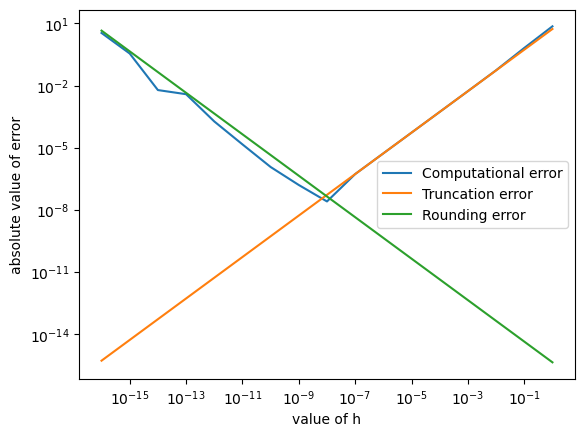
\includegraphics[width=0.67\textwidth]{img/deriv_right_err.png}
	}
	\caption{Wykres wspólny wartości bezwględnych błędów - różnica prawostronna}
	\label{zad1:graph1}
\end{figure}

Zauważmy, że wykresy błędów zachowują się zgodnie z~przewidywaniami opartymi na zależności~(\ref{zad1:eqn4}). Ponadto można stwierdzić, że wykres błędu obliczeniowego ma w~pewnym punkcie minimum - mianowicie w~$10^{-8}$, natomiast należy wziąć poprawkę na fakt, że punkty wykresu zostały połączone prostymi liniami, aby zwiększyć czytelność. Poniżej przedstawiamy obliczenia prowadzące do wyznaczenia dokładnej wartości $h_{min}$, dla której prawa strona nierówności~(\ref{zad1:eqn4}) przyjmuje najmniejszą wartość. Mamy zatem

\begin{align}
	\frac{\partial{(\frac{Mh}{2}+\frac{2\epsilon}{h}})}{\partial{h}} &= 0 \\
	\frac{M}{2}-\frac{2\epsilon}{h^2} &= 0 \\
	h^2 &= \frac{4\epsilon}{M} \\ 
	h_{min} = h &= 2\sqrt{\frac{\epsilon}{M}}
\end{align}
Podstawiając wartości $\epsilon$~i~$M$, uzyskujemy $h_{min} \approx 9.123695 \cdot 10^{-9}$.

Przejdźmy zatem do obliczenia wartości bezwględnej błędu względnego (obliczeniowego) w~punkcie~$h_{min}$. Wyliczamy ją ze wzoru $\left| \frac{E(h_{min})}{tan'(1)} \right|$ i~otrzymujemy 
$$
\left| \frac{E(h_{min})}{tan'(1)} \right| \approx 5.33866349 \cdot 10^{-9}
$$.

\newpage

\subsection{Podejście drugie - różnica centralna}

Przy tym podejściu zachodzi zależność \footnote{Wzór zaczerpnięty z~\cite{teams_materials}.}

\begin{equation}
	E(h) \le \frac{Mh^2}{6}+\frac{\epsilon}{h},
	\label{zad1:eqn9}
\end{equation}
gdzie:

\begin{itemize}
	\item błąd metody jest wyrażony wzorem $\frac{Mh^2}{6}$ i~w~tym przypadku $M \approx 56.7029999$, 
	\item błąd numeryczny to $\frac{\epsilon}{h}$ ($\epsilon$ ma taką samą wartość jak w~pierwszym podejściu),
	\item błąd obliczeniowy $E(h)$ jest, tak jak poprzednio, różnicą między uzyskanym wynikiem a~wartością obliczoną ze wzoru~(\ref{zad1:eqn3}).
\end{itemize}
Przedstawiamy wykresy wartości bezwzględnych błędów na wspólnym wykresie, przy czym na obu osiach użyto skali logarytmicznej.

\begin{figure}[h!]
	\centering{
		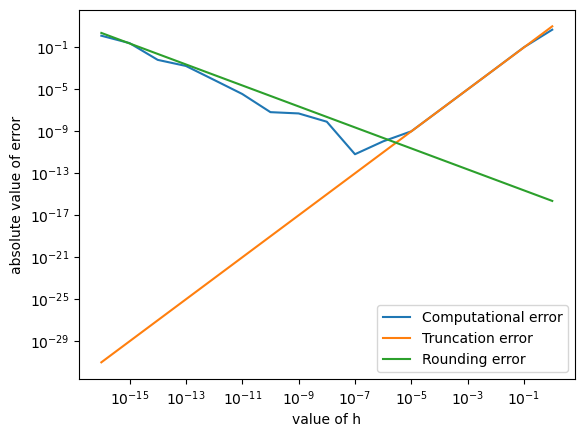
\includegraphics[width=0.67\textwidth]{img/deriv_central_err.png}
	}
	\caption{Wykres wspólny wartości bezwględnych błędów - różnica centralna}
	\label{zad1:graph2}
\end{figure}

Podobnie jak w~pierwszym podejściu, tutaj także wykresy zachowują się zgodnie z~przewidywaniami wedle zależności~(\ref{zad1:eqn9}) oraz wykres błędu obliczeniowego ma w~pewnym punkcie minimum, które tym razem graficznie przypada w~$10^{-7}$. Poniżej przedstawiamy obliczenia prowadzące do wyznaczenia dokładnej wartości $h_{min}$, dla której prawa strona nierówności~(\ref{zad1:eqn9}) przyjmuje najmniejszą wartość. Mamy zatem

\begin{align}
	\frac{\partial{(\frac{Mh^2}{6}+\frac{\epsilon}{h}})}{\partial{h}} &= 0 \\
	\frac{Mh}{3}-\frac{\epsilon}{h^2} &= 0 \\
	h^3 &= \frac{3\epsilon}{M} \\ 
	h_{min} = h &= \sqrt[3]{\frac{3\epsilon}{M}}
\end{align}
Podstawiając wartości $\epsilon$~i~$M$, uzyskujemy $h_{min} \approx 2.273274 \cdot 10^{-6}$.

Możemy teraz obliczyć wartość bezwględną błędu względnego w~wyznaczonym punkcie~$h_{min}$. Postępując analogicznie, w~tym przypadku wynosi ona $\approx 2.53340126 \cdot 10^{-11}$.

\newpage
